% !TeX root = ../main.tex
% Optional. Jeder Anhangsabschnitt braucht mindestens eine Referenz aus dem
% Fließtext (\autoref{sec:anhang-...}), sonst ist er ein Vorgabenverstoß.
\appendix
\chapter{Anhang}
\label{cha:anhang}

\section{Beispiel eines Programmablaufplans}
\label{sec:anhang-pap}

\begin{figure}[H]
    \centering
    % Quelle: assets/diagrams/programmablaufplan.md (Mermaid)
    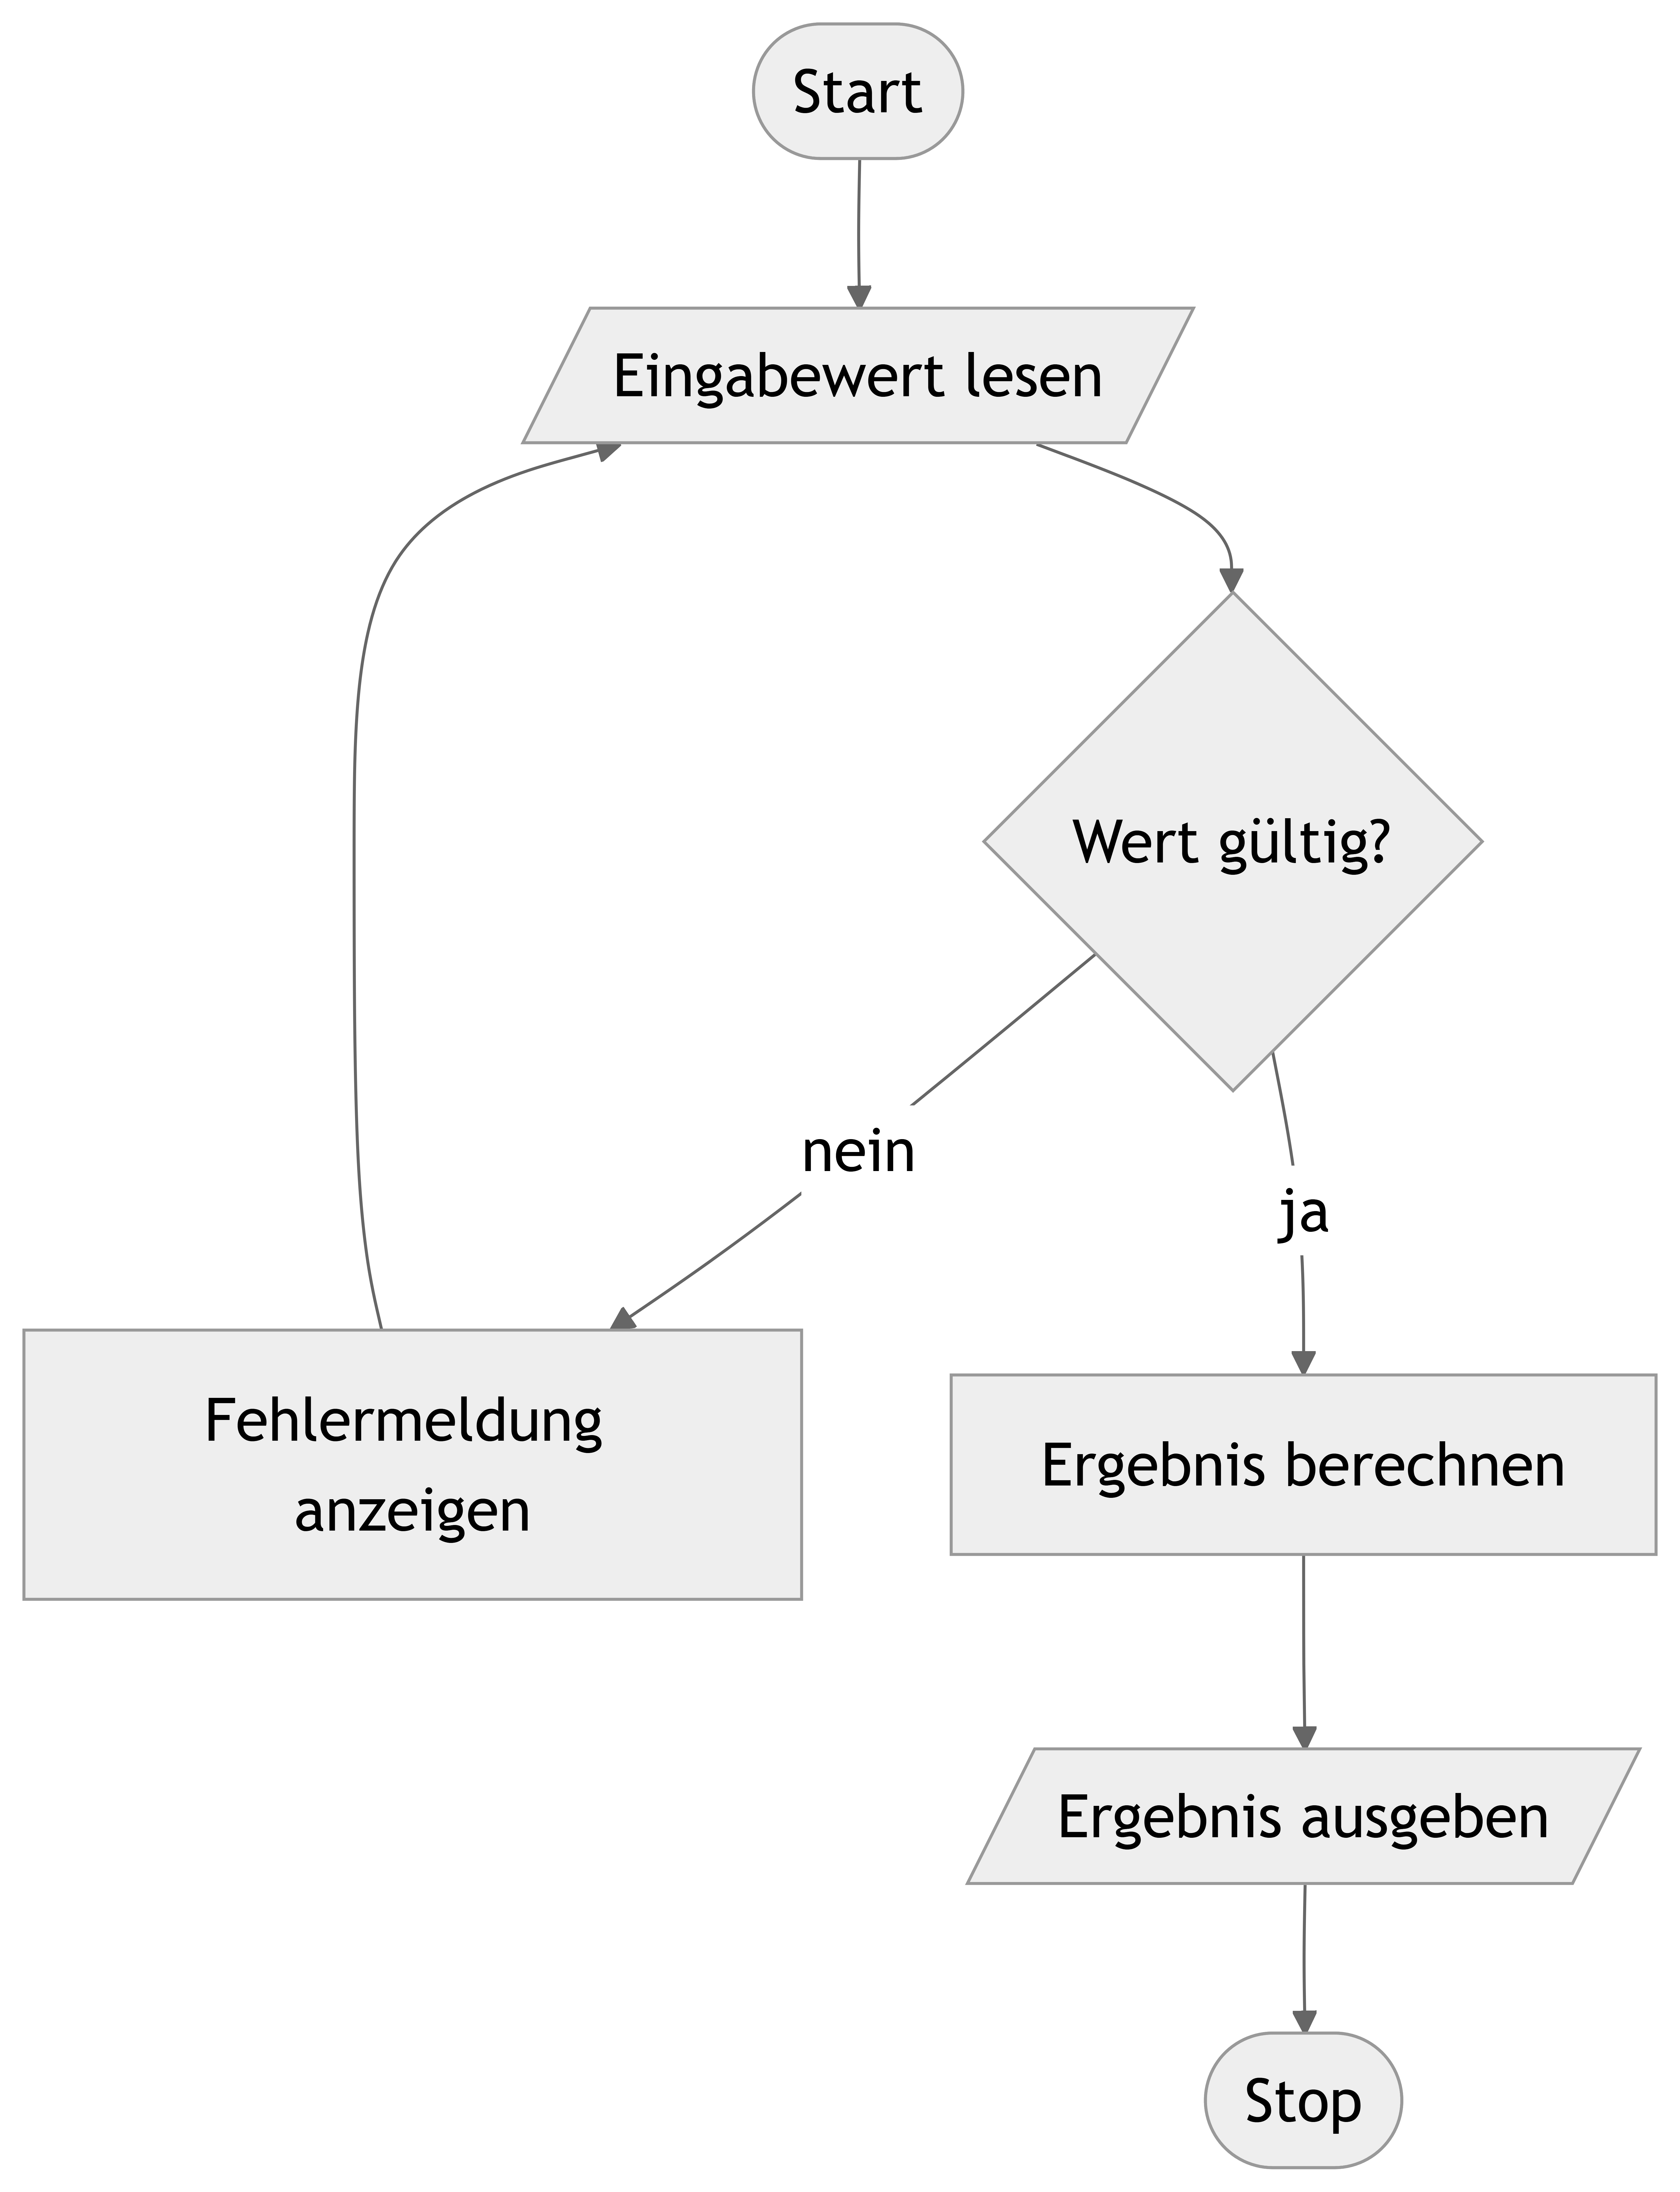
\includegraphics[width=0.6\textwidth]{assets/diagrams/programmablaufplan.png}
    \caption{Programmablaufplan nach DIN~66001 (Beispiel)}
    \label{fig:pap-beispiel}
\end{figure}
